\documentclass[a4paper,10pt]{book}

%\usepackage{graphicx}
\usepackage{color}
\usepackage{bm}
\usepackage{amsmath}
\usepackage{appendix}
\usepackage{xspace}
\usepackage{a4wide}
%\usepackage{hyperref}
\usepackage{wrapfig}
\usepackage[numbers,comma,sort&compress]{natbib}
\usepackage{graphicx}
\usepackage{xstring}
\usepackage{listings,xcolor,courier}

\usepackage
[dvips, %or dvips or pdftex
pagebackref, %or backref
colorlinks=true,
linkcolor=webgreen, %defined below
filecolor=webbrown, %defined below
citecolor=webgreen, %defined below
pdftitle={VOTCA manual},
pdfauthor={},
pdfsubject={VOTCA},
pdfkeywords={coarse-graining boltzmann inversion monte carlo force matching},
bookmarksopen=false,
pdfpagemode=UseNone]{hyperref}

\definecolor{webgreen}{rgb}{0,.5,0}
\definecolor{webbrown}{rgb}{.6,0,0}
\pdfcompresslevel=9

\renewcommand{\vec}[1]{\ensuremath{{\bm #1}}}
\newcommand{\fig}[1]{fig.~\ref{#1}}
\newcommand{\eq}[1]{eq.~\ref{#1}}
\newcommand{\unit}[1]{\ensuremath{\,\mbox{#1}}}
\newcommand{\ibi}{IBI\xspace}
\newcommand{\imc}{IMC\xspace}
\newcommand{\fm}{FM\xspace}
\newcommand{\xml}{XML\xspace}
\newcommand{\gromacs}{GROMACS\xspace}
\newcommand{\spce}{SPC/E\xspace}
\newcommand{\grad}{\vec{\nabla}}
\newcommand{\ddash}{{-}{-}\xspace}

%formating for a program option, e.g. --trj
\newcommand{\progopt}[1]{\texttt{#1}\xspace}
% formating for programs, e.g. csg_boltzmann
\newcommand{\prog}[1]{\hyperref[#1]{\textbf{\StrSubstitute{#1}{_}{\_}}}\xspace}
% formating for an xml option, e.g. cg.inverse.simprog
\newcommand{\xmlopt}[1]{\textit{#1}\xspace}

% reference to an xml option in the reference section
\newcommand{\cgref}[1]{cg.#1}
\newcommand{\interref}[1]{cg.interaction.#1}
\newcommand{\mapref}[1]{mapping.#1}


\newcommand{\sect}[1]{sec.~\ref{#1}}

\newcommand{\votca}{{\sc \color{blue} votca}\xspace}
\newcommand{\votcaweb}{\htmladdnormallink{{\sc \color{blue} www.votca.org}\xspace}{http://www.votca.org}}


\newcommand{\sasha}{ {\sc \color{red} Alexander Lukyanov} \newline}
\newcommand{\denis}{ {\sc \color{red} Denis Andrienko} \newline}
\newcommand{\victor}{ {\sc \color{red} Victor R\"uhle} \newline}
\newcommand{\christoph}{ {\sc \color{red} Christoph Junghans} \newline}

%\usepackage[T1]{fontenc}
%\usepackage{times}
\usepackage{type1cm}

% XML listings
\definecolor{darkgreen}{named}{green}
\definecolor{darkblue}{named}{blue}
\definecolor{darkred}{named}{red}
\definecolor{grau}{named}{gray}
\let\Righttorque\relax

\lstset{language=XML}
% \lstset{
% commentstyle=\itshape\color{darkgreen},
% keywordstyle=\bfseries\color{darkblue},
% stringstyle=\color{darkred},
% extendedchars=true,
% basicstyle=\scriptsize\ttfamily
% basicstyle=\tiny\ttfamily,
% tabsize=2,
% % keywordstyle=\textbf,
% commentstyle=\color{grau},
% % stringstyle=\textit,
% numbers=left,
% numberstyle=\tiny,
% % für schönen Zeilenumbruch
% breakautoindent = true,
% breakindent = 2em,
% breaklines = true,
% postbreak = ,
% prebreak = \raisebox{-.8ex}[0ex][0ex]{\ensuremath{\lrcorner}},
% prebreak = \raisebox{-.8ex}[0ex][0ex]{\Righttorque},
% showspaces=false, % Keine Leerzeichensymbole
% showtabs=false, % Keine Tabsymbole
% showstringspaces=false,% Leerzeichen in Strings
% }

\lstset{
    language=XML,
    basicstyle=\ttfamily\scriptsize\mdseries,
    keywordstyle=\bfseries\color{darkblue},
    identifierstyle=,
    commentstyle=\color{gray},  
    stringstyle=\itshape\color{darkred},
    breaklines=true,
    frame=none,
    showstringspaces=false,
    tabsize=4,
    captionpos=b,
    float=htbp,
%    keywords={name,cg,fmatch,frames_per_block,non-bonded,
%       type1,type2,min,max,step,out_step,non-bonded,ident,cg_beads,cg_bead,topology,map,bond,cg_bonded,
%       angle,beads,maps,weights,cg_molecule,molecules,rename,clear,define,mapping,type,non-bonded,bonded,constraintedLS,
%       post_update,smooth,iterations,type},
    morecomment=[s]{!--}{--}
}


\begin{document}
\frontmatter
\input{hgid}
\begin{titlepage}

\center{\fontsize{4cm}{5cm}\selectfont VOTCA}
\center{\fontsize{1.5cm}{3cm}\selectfont USER MANUAL}

\vspace*{3cm}
\center{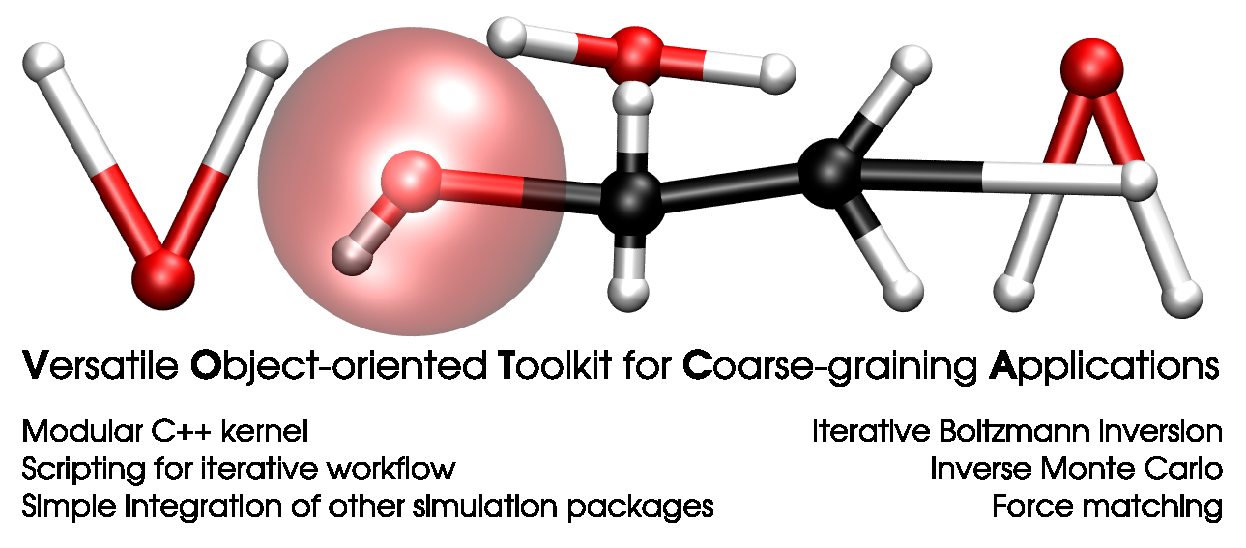
\includegraphics[width=\columnwidth]{fig/logo}}
\vspace*{1cm}

\center{\Large{Victor R\"uhle}}
\center{\Large{Christoph Junghans}}
\center{\Large{Alexander Lukyanov}}
\center{\Large{Kurt Kremer}}
\center{\Large{Denis Andrienko}}

\vspace*{1.4cm}
\center{\large{\today}}
\vspace*{-0.3cm}
\center{\footnotesize{compiled from: \hgid}}
\center{\footnotesize{Programs version: \refhgid}}

\vspace*{1cm}
%\center{
\large{\copyright \hspace*{0.1cm} VOTCA development team}
%}
\vspace*{0.5cm}

\htmladdnormallink{\color{black}\large{www.votca.org}}{http://www.votca.org}
\end{titlepage}

\thispagestyle{empty}
\cleardoublepage

\tableofcontents
\cleardoublepage
\mainmatter
\chapter{Introduction}
\label{sec:introduction}
%\denis

Versatile Object-oriented Toolkit for Coarse-graining Applications, or \votca, is a package which helps to systematically coarse-grain various systems~\cite{Ruehle:2009.a}. This includes  deriving the coarse-grained potentials, assessing their quality, preparing input files required for coarse-grained simulations, and analyzing the latter.

A typical coarse-graining workflow includes {\em sampling} of the system of interest, {\em analysis} of the trajectory using a specific {\em mapping} and a coarse-graining {\em method} to derive coarse-grained potentials and, in case of iterative methods, running coarse-grained simulations and iteratively {\em refining} the coarse-grained potentials.

In most cases, coarse-graining requires canonical sampling of a reference (high resolution) system. In addition, iterative methods require canonical sampling of the coarse-grained system. The sampling can be done using either molecular dynamics (MD), stochastic dynamics (SD), or Monte Carlo (MC) techniques. The latter are implemented in many standard simulation packages. Rather than implementing its own MD/SD/MC modules, \votca allows swift and flexible integration of existing  programs in such a way that sampling is performed by the program of choice. At the moment, an interface to \gromacs~\cite{gromacs4} simulation package is provided. The rest of the analysis needed for systematic coarse-graining is done using the package tools.

\begin{wrapfigure}{ht}{4cm}
 \includegraphics[width=4cm]{fig/propane}
 \caption{\small Three-bead coarse-grained model of propane.
 \label{fig:intro:propane}
}
\end{wrapfigure}

The workflow can be exemplified on coarse-graining of a propane liquid. A single molecule of propane contains three carbon and eight hydrogen atoms. A united atom coarse-grained representation of a propane molecule has three beads and two bead types, A and B, with three and two hydrogens combined with the corresponding atom, as shown in \fig{fig:intro:propane}. This representation defines the \hyperref[sec:mapping_operator]{mapping operator}, as well as the bonded coarse-grained degrees of freedom, such as the bond $b$ and the bond angle $\theta$. Apart from the bonded interactions, $u_b$ and $u_\theta$, beads belonging to different molecules have non-bonded interactions, $u_\text{AA}$, $u_\text{AB}$, $u_\text{BB}$. The task of coarse-graining is then to derive a potential energy surface $u$ which is a function of all coarse-grained degrees of freedom. Note that, while the atomistic bond and angle potentials are often chosen to be simple harmonic functions, the coarse-grained potentials cannot be expressed in terms of simple analytic functions. Instead, tabulated functions are normally used.

The coarse-graining {\em method} defines criteria according to which the potential energy surface is constructed. For example, for the bond $b$ and the angle $\theta$~\hyperref[sec:bi]{Boltzmann Inversion} can be used. In this case a coarse-grained potential will be a potential of mean force. For the non-bonded degrees of freedom, the package provides \hyperref[sec:ibi]{Iterative Boltzmann Inversion (\ibi)} or \hyperref[sec:imc]{Inverse Monte Carlo (\imc)} methods. In this case the radial distribution functions of the coarse-grained model will match those of the atomistic model. Alternatively, \hyperref[sec:fm]{Force Matching (\fm)} (or multiscale coarse-graining) can be used, in which case the coarse-grained potential will approximate the many-body potential of mean force. The choice of a particular method is system-specific and requires a thorough consistency check. It is important to keep in mind that coarse-graining should be used with understanding and caution, methods should be crossed-checked with each other as well as with respect to the reference system.

The package consists of two parts: a C++ kernel and a scripting engine. The kernel is capable of processing atomistic topologies and trajectories and offers a flexible framework for reading, manipulating and analyzing topologies and generated by MD/SD/MC sampling trajectories. It is modular: new file formats can be integrated without changing the existing code. Currently, an interface for \gromacs~\cite{gromacs4} topologies and trajectories is provided.
%
The kernel also includes various coarse-graining tools, for example calculations of probability distributions of bonded and non-bonded interactions, correlation and autocorrelation functions, and updates for the coarse-grained pair potential.

The scripting engine is used to steer the iterative procedures. Here the analysis tools of the package used for sampling (e.g. \gromacs tools) can be integrated into the coarse-graining workflow, if needed. The coarse-graining workflow itself is controlled by several Extensible Markup Language (\xml) input files, which contain mapping and other options required for the workflow control. In what follows, these input files are described.

Before using the package, do not forget to initalize the variables in the bash or csh (tcsh)
\begin{verbatim}
  source <csg-installation>/bin/VOTCARC.bash
  source <csg-installation>/bin/VOTCARC.csh
\end{verbatim}

More details as well as several examples can be found in ref.~\cite{Ruehle:2009.a}. Please cite this paper if you are using the package. Tutorials can be found on the \votca homepage \votcaweb.

\chapter{Theoretical background}

\section{Mapping}
\label{sec:mapping_operator}
%\sasha
%mapping scheme ($c_{Ii}$ coefficients) \\
%TO DO: picture \\
%translation invariance \\
%definition of the mass \\
%definition of specific and involved atoms \\

The mapping is an operator that establishes a link between the atomistic and coarse-grained representations of the system. An atomistic system is described by specifying the values of the Cartesian coordinates and momenta
\begin{eqnarray}
\bm r^n &=& \{\bm r_1,\dots,\bm r_n\}, \\
\bm p^n &=& \{\bm p_1,\dots,\bm p_n\}.
\end{eqnarray}
of the $n$ atoms in the system.\footnote{In what follows we adopt notations of ref.~\cite{Noid:2008.1}.}
%
On a coarse-grained level, the coordinates and momenta are specified by the positions and momenta of CG sites
\begin{eqnarray}
\bm R^N = \{\bm R_1,\dots,\bm R_N\}, \\
\bm P^N = \{\bm P_1,\dots,\bm P_N\}.
\end{eqnarray}
Note that capitalized symbols are used for the CG sites while lower case letters are used for the atomistic system.

The mapping operator defined by a matrix for each bead $I$, ${\bm c}_I$, then links the two descriptions
\begin{eqnarray}
 {\bm R}_I &=& \sum_{i=1}^{n}c_{Ii}\bm r_i, \\
 {\bm P}_I &=&
 	M_I \dot{{\bm R}}_I =
	M_I \sum_{i=1}^{n}c_{Ii} \dot{{\bm r}}_i =
	M_I \sum_{i=1}^{n} \frac{ c_{Ii}} {m_i} {\bm p}_i .
\label{eq:mapping_scheme}
\end{eqnarray}
for all $I = 1,\dots,N$.

If an atomistic system is translated by a constant vector, the corresponding coarse-grained system is also translated by the same vector. This implies that, for all $I$,
\begin{equation}
 \sum_{i=1}^{n}c_{Ii}=1.
\end{equation}

In some cases it is useful to define CG mapping in a way that certain atoms belong to several CG beads at the same time~\cite{Fritz:2009}. Following ref.~\cite{Noid:2008.1} we define two sets of atoms for each of the $N$ CG beads. For each site $I$, a set of {\em involved} atoms is defined as
\begin{equation}
 {\cal I}_I=\{i|c_{Ii}\ne0\}.
\end{equation}
An atom $i$ in the atomistic model is involved in a CG site, \textit{I}, if and only if this atom provides a nonzero contribution to the sum in eq.~\ref{eq:mapping_scheme}.

A set of {\em specific} atoms is defined as
\begin{equation}
 {\cal S}_I=\{i|c_{Ii}\ne0 \text{ and } c_{Ji}=0 \text{ for all } J \ne I\}.
\end{equation}
In other words, atom $i$ is specific to site $I$ if and only if this atom is involved in site $I$ and is not involved in the definition of any other site.

The CG model will generate an equilibrium distribution of momenta that is consistent with an underlying atomistic model if all the atoms are {\em specific} and if the mass of the $I^\text{th}$ CG site is given by~\cite{Noid:2008.1}
\begin{equation}
M_I= \left( \sum_{i \in {\cal I}_I}\frac{c_{Ii}^2}{m_i} \right)^{-1}.
\label{eq:cg_mass}
\end{equation}
%
If all atoms are specific and the center of mass of a bead is used for mapping, then $c_{Ii} = \frac{m_i}{M_I}$, and the condition~\ref{eq:cg_mass} is automatically satisfied.

%%%%%%%%%%%%%%%%%%%%%%%%%%%%%%%%%%%%%%%%%%%%%%%%%%%%%%%%%%%%%%%%%%%%%%%%%%%%%%%%%
\section{Boltzmann inversion}
\label{sec:bi}

Boltzmann inversion is mostly used for {\em bonded} potentials, such as bonds, angles, and torsions~\cite{Tschoep:1998}. Boltzmann inversion is structure-based and only requires positions of atoms.

The idea of Boltzmann inversion stems from the fact that in a canonical ensemble {\em independent} degrees of freedom $q$ obey the Boltzmann distribution, i.~e.
%
\begin{equation}
  P(q) = Z^{-1} \exp\left[ - \beta U(q) \right]~,
  \label{eq:boltzmann}
\end{equation}
%
where \mbox{$Z = \int \exp \left[ - \beta U(q) \right] \text{d}q $} is a partition function, \mbox{$\beta = 1/k_\text{B} T$}.
%
Once $P(q)$ is known one can obtain the coarse-grained potential, which in this case is a potential of mean force, by inverting the probability distribution $P(q)$ of a variable $q$, which is either a bond length, bond angle, or torsion angle
\begin{equation}
  U(q) = - k_\text{B} T \ln  P(q) ~.
  \label{eq:inv_boltzmann}
\end{equation}
%
The normalization factor $Z$ is not important since it would only enter the coarse-grained potential $U(q)$ as an irrelevant additive constant.

Note that the histograms for the bonds $H_r(r)$, angles $H_\theta(\theta)$, and torsion angles $H_\varphi(\varphi)$ have to be rescaled in order to obtain the volume normalized distribution functions $P_r(r)$, $P_\theta(\theta)$, and $P_\varphi(\varphi)$, respectively
%
\begin{align}
    P_r(r) = \frac{H_r(r)}{4\pi r^2}~,\;
    P_\theta(\theta) = \frac{H_\theta(\theta)}{\sin \theta}~,\;
    P_\varphi(\varphi) = H_\varphi (\varphi)~,
    \label{eq:boltzmann_norm}
\end{align}
where $r$ is the bond length $r$, $\theta$ is the bond angle, and $\varphi$ is the torsion angle. The bonded coarse-grained potential can then be written as a sum the distribution functions
%
\begin{align}
    \label{eq:boltzmann_pmf}
    U({r}, \theta, \varphi) &= U_r({r}) + U_{\theta}(\theta) + U_{\varphi}(\varphi)~, \\
    U_q({q}) &= - k_\text{B} T \ln P_q( q ),\; q=r, \theta, \varphi~.
    \nonumber
\end{align}

On the technical side, the implementation of the Boltzmann inversion method requires {\em smoothing} of $U(q)$ to provide a continuous force. Splines can be used for this purpose. Poorly and unsampled regions, that is regions with high $U(q)$, shall be {\em extrapolated}. Since the contribution of these regions to the canonical density of states is small the exact shape of the extrapolation is less important.

Another crucial issue is the cross-correlation of the coarse-grained degrees of freedom. Independence of the coarse-grained degrees of freedom is the main assumption that allows factorization of the probability distribution and the potential, eq.~\ref{eq:boltzmann_pmf}. Hence, one has to carefully check whether this assumption holds in practice. This can be done by performing coarse-grained simulations and comparing cross-correlations for all pairs of degrees of freedom in atomistic and coarse-grained resolution, e.~g. using a two-dimensional histogram, analogous to a Ramachandran plot.~\footnote{Checking the linear correlation coefficient does not guarantee statistical independence of variables, for example $c(x, x^2)=0$ if $x$ has a symmetric probability density $P(x) = P(-x)$. This case is often encountered in systems used for coarse-graining.}

\subsection{Separation of bonded and non-bonded degrees of freedom}
When coarse-graining polymeric systems, it is convenient to treat bonded and non-bonded interactions separately~\cite{Tschoep:1998}. In this case, sampling of the atomistic system shall be performed on a special system where non-bonded interactions are artificially removed, so that the non-bonded interactions in the reference system do not contribute to the bonded interactions of the coarse-grained model.

This can be done by using exclusion lists using \prog{csg_boltzmann} with the option \progopt{--excl}. This is describe in detail in sec. \ref{sec:exclusions}.


%%%%%%%%%%%%%%%%%%%%%%%%%%%%%%%%%%%%%%%%%%%%%%%%%%%%%%%%%%%%%%%%%%%%%%%%%%%%%%%%%%%%%%%%%%%%%%%%
\section{Iterative Boltzmann Inversion}
\label{sec:ibi}

Iterative Boltzmann inversion (\ibi) is a natural extension of the Boltzmann inversion method. Since the goal of the coarse-grained model is to reproduce the distribution functions of the reference system as accurately as possible, one can also iteratively refine the coarse-grained potentials using some numerical scheme.

In \ibi the potential update $\Delta U$ is given by~\cite{Reith:2003}
\begin{eqnarray}
  \label{eq:iter_boltzmann}
  U^{(n+1)} &=& U^{(n)} + \lambda \Delta U^{(n)}~, \\
  \Delta U^{(n)} &=&  k_\text{B} T \ln  \frac{P^{(n)}}{P_{\rm ref}}
  =  U_\text{PMF}^\text{ref} - U_\text{PMF}^{(n)}~.
\end{eqnarray}
Here $\lambda \in (0,1]$ is a numerical factor which helps to stabilize the scheme.

The convergence is reached as soon as the distribution function $P^{(n)}$ matches the reference distribution function $P_{\rm ref}$, or, in other words, the potential of mean force, $U_\text{PMF}^{(n)}$ converges to the reference potential of mean force.

\ibi can be used to refine both bonded and non-bonded potentials. It is primarily used for simple fluids with the aim of reproducing the radial distribution function of the reference system in order to obtain non-bonded interactions. On the implementation side, \ibi has the same issues as the inverse Boltzmann method, i.~e. smoothing and extrapolation of the potential must be used.


\section{Inverse Monte Carlo}
\label{sec:imc}

Inverse Monte Carlo (\imc) is an iterative scheme which additionally includes cross correlations of distributions. A detailed derivation of the \imc method can be found in ref.~\cite{Lyubartsev:1995}.

The potential update $\Delta U$ of the \imc method is calculated by solving a set of linear equations
\begin{align}
    \left<S_{\alpha}\right> - S_{\alpha}^{\text{ref}}= A_{\alpha \gamma} \Delta U_{\gamma}~,
  \label{eq:imc}
\end{align}
%
where
\begin{eqnarray}
  \label{eq:covariance}
  A_{\alpha \gamma} = \frac{\partial \left< S_{\alpha} \right> }{\partial U_{\gamma}}  =
  \beta \left( \left<S_{\alpha} \right>\left<S_{\gamma} \right> - \left<S_{\alpha} S_{\gamma} \right>  \right)~,
  \nonumber
\end{eqnarray}
and $S$ the histogram of a coarse-grained variable of interest. For example, in case of coarse-graining of the non-bonded interactions which depend only on the distance, $r_{ij}$, between particles $i$ and $j$ and assuming that the interaction potential is short-ranged, i.e. $U(r_{ij})=0$ if $r_{ij} \ge r_{\text{cut} }$, the average value of $S_{\alpha}$ is related to the radial distribution function $g(r_{\alpha})$
%
\begin{equation}
   \left< S_{\alpha} \right> =  \frac{N(N-1)}{2} \frac{4 \pi r_{\alpha}^2 \Delta r} {V}g(r_{\alpha})~,
  \label{eq:s_mean}
\end{equation}
%
where $N$ is the number of atoms in the system ($\frac{1}{2} N(N-1)$ is then the number of all pairs), $\Delta r$ is the grid spacing, $r_{\text{cut}}/M$, $V$ is the total volume of the system. In other words, in this particular case the physical meaning of $S_{\alpha}$ is the number of particle pairs with interparticle distances $r_{ij} = r_{\alpha}$ which correspond to the tabulated value of the potential $U_{\alpha}$.


\section{Force Matching}
\label{sec:fm}

%\sasha

%Brief description with references \\
% Maybe appendix with main equations \\

Force matching (\fm) is another approach to evaluate corse-grained potentials~\cite{Ercolessi:1994,Izvekov:2005,Noid:2007}. In contrast to the structure-based approaches, its aim is not to reproduce various distribution functions, but instead to match the multibody potential of mean force as close as possible with a given set of coarse-grained interactions.

The method works as follows. We first assume that the coarse-grained force-field (and hence the forces) depends on $M$ parameters $g_1,...,g_M $. These parameters can be prefactors of analytical functions, tabulated values of the interaction potentials, or coefficients of splines used to describe these potentials.

In order to determine these parameters, the reference forces on coarse-grained beads are calculated by summing up the forces on the atoms
\begin{equation}
  {\vec F}_I^\text{ref} = \sum_{j \in {\cal S_I}} \frac{d_{Ii}}{c_{Ii}} {\vec f}_j({\vec r^n}),
  \label{eq:force_mapping}
\end{equation}
where the sum goes over all atoms of the CG site {\it I} (see. \sect{sec:mapping_operator}).
The $d_{Ij}$ coefficients can, in principle, be chosen arbitrary, provided that the condition $ \sum_{i=1}^{n}d_{Ii}=1$ is sutisfied~\cite{Noid:2008.1}. If mapping coefficients for the forces are not provided, it is assumed that $d_{Ij} = c_{Ij}$ (see also \sect{sec:mapping}).

By calculating the reference forces for $L$ snapshots we can write down $N \times L$ equations
%
\begin{equation}
  {\vec F}_{Il}^\text{cg}(g_1, \dots ,g_M)=\vec F_{il}^\text{ref},\;
  I=1,\dots,N,\; l=1,\dots,L~.
  \label{eq:fmatch1}
\end{equation}
%
Here ${\vec F}_{Il}^\text{ref}$ is the force on the bead $I$, ${\vec F}_{Il}^\text{cg} $ is the coarse-grained representation of this force. Index $l$ enumerates snapshots picked for coarse-graining. By running the simulations long enough one can always ensure that $M < N \times L$. In this case the set of equations~\ref{eq:fmatch1} is overdetermined and can be solved in a least-squares manner.

${\bm F}_{il}^\text{cg}$ is, in principle, a non-linear function of its parameters $\{g_i\}$. It is, therefore, useful to represent the coarse-grained force-field in such a way that equations~(\ref{eq:fmatch1}) become linear functions of $\{g_i\}$. This can be done using splines to describe the functional form of the forces~\cite{Izvekov:2005}. Implementation details are discussed in ref.~\cite{Ruehle:2009.a}.

Note that an adequate sampling of the system requires a large number of snapshots $L$. Hence, the applicability of the method is often constrained by the amount of memory available. To remedy the situation, one can split the trajectory into blocks, find the coarse-grained potential for each block and then perform averaging over the blocks.

\chapter{Implementation}
\subsection{Coarse-graining engine}
\votca can be divided into two main parts. A C++ kernel, which includes various coarse-graining tools and is capable of processing topologies and trajectories, and a scripting enginge to steers the iterative procedures.

These tools include calculations of probability distributions of bonded and non-bonded interactions, correlation and autocorrelation functions, and updates for the coarse-grained pair potential. Analysis tools of the MD package can also be integrated into the coarse-graining workflow, as needed.

The package offers a flexible framework for reading, manipulating and analyzing of MD/SD/MC topologies and trajectories. Its core is modular and new file formats can be integrated without changing the existing code. Currently, an interface for \gromacs~\cite{gromacs4} topologies and trajectories is provided.

The coarse-graining procedure itself is controlled by several Extensible Markup Language (\xml) input files, which contain mapping and other options required for the workflow control. For the mapping, it is possible to select groups of interactions which are used for the coarse-graininged analysis. 
%It is possible to generate exclusion lists for Boltzmann inversion of bonded interactions or virtual sites for back-mapping.

\section{Mapping}
\label{sec:mapping}
{\em Mapping definitions} describe how to map a single molecule from an atomistic to a coarse-grained representation. A mapping definition has to be specified only once per molecule. The file contains sections for coarse-grained beads, bonded interactions in the coarse grained scheme as well as mapping matrices. If a system contains several molecule types, it has to be enssured that molecule names are set properly. The mapping files should be specified in a list separated by ; (e.g. "protein.xml;solvent.xml"). The \mapopt{ident} tag in the mapping definition must match the name of the molecule in the reference system.

The mapping file has similar entries as a topology, but contains additional information for mapping are present. In the topology section, coarse grained beads and bonded interactions are defined. Each coarse grained bead has a name, type and mapping entry, as well as a list of atoms which are mapped to it. The name must be unique within the mapping file. Type defines the type of the bead. The \mapopt{mapping} tag defines which mapping scheme is used from the mapping section in the file. Type and mapping can be different since the number of atoms for the same bead type may differ, e.g. at chain ends for saturating hydrogen atoms.

In the \mapopt{mapping} section, the mapping operator is defined. Currently this includes only weights for a linear mapping scheme.

A complete reference for mapping file definitions can be found in ref.~\ref{sec:ref_mapping}. To map from an atomistic to a reference system, \textbf{csg\_map} can be used:
\begin{verbatim}
  csg_map --top topol.tpr --trj traj.trr --cg "protein.xml;solvent.xml" --out cg.gro
\end{verbatim}

To create a coarse-grained topology based on the mapping scheme, see \textbf{csg\_gmxtopol}.

\subsection{Example - mapping file for propane}
\begin{figure}[ht]
  \includegraphics[width=0.4\textwidth]{functionality/fig/propane.eps}
  \caption{Mapping for propane}
\end{figure}

\lstinputlisting{functionality/propane.xml}


\section{Topologies}
A topology is defined as a set of beads with a certain bead type which are connected by bonded interactions.
Votca can read topologies in the \gromacs tpr format. Additionally, it can use a pdb file as topology, however, not all information are given in a pdb file and are not defined. If a pdb topology is used, it is recommended to fill additional molecule information using the xml advanced topology handling feature (see. \sect{sec:adv_topology})
\subsection{Manual topology handling}
\label{sec:adv_topology}
Many file formats do not have a clear definition of a molecules. This can lead to problems, especially if a simulation contains several multiple molecules. Since during the coarse graining, the molecule type is identified by a name tag, names must be set properly. \votca offers the possibility to read a topology and later on modify parts of it. Everything is defined in an xml topology file.

Also \gromacs did not store molecule names in previous versions. This was introduced in a newer release. If possible, always provide a recent .tpr file which contains molecule names. For old topologies, rerun grompp if possible to get a recent file.

If a system with multiple molecule types is processed, but no molecule names are present, molecule names have to be specified manually as described in this section that \votca can choose the correct mapping scheme..

If no molecule information is present at all, they can be created. An for a topology file that reads in last.pdb and then creates molecules is:
\begin{verbatim}
<topology base="last.pdb">
  <molecules>
    <clear/>
    <define name="mCP" first="1" nbeads="52" nmols="216"/>
  </molecules>
</topology>
\end{verbatim}
<clear/> clears all bolecule information that were present before.

If the file format the topology is read from only does not support molecules names, \votca offers the possibility to define topologies in an xml file and manipulate the molecule names after reading. A short example:
\begin{verbatim}
 <topology base="topol.tpr">
   <molecules>
     <rename name="PPY3" range="1:125"/>
     <rename name="Cl" range="126:250"/>
   </molecules>
 </topology>
\end{verbatim}
Here, first to file topol.tpr is loaded. The file supports molecules but does not give a name tag. Afterwards, Molecules are renamed. This file can be loaded as any other topology.

To use the new topology, create a file using the schema above and save it as .xml. To use it in the program, you'll have to give several coarse graining definitions, separated by ;. If you saved the example above as newtop.xml, use 

\subsection{Trajectories}
A trajectory is defined as a set of frames containing coordinates and eventually velecities and forces for the beads of a topology.
VOTCA currently supports trr, xtc, pdb and gro as trajector formats.

\section{Iterative workflow control}

\begin{figure}
  \includegraphics[width=0.7\columnwidth]{functionality/fig/flowchart.eps}
  \caption{
    \label{fig:flowchart}
    Block-scheme of the workflow control for the iterative methods. The most time-consuming parts are marked in red.
  }
\end{figure}

During the global initialization the initial guess for the coarse-grained potential is calculated from the reference radial distribution function or converted from a given potential guess to the internal format. The actual iterative step starts with an iteration initialization. It searches for possible checkpoints and copies and converts files from the previous step and the base directory. Then the simulation run is prepared by converting potentials to the format required by the external sampling program and the actual sampling is performed. Currently, an interface with \gromacs~\cite{gromacs4} is implemented but an extension for other packages is straightforward. After sampling the phasespace, the potential update $\Delta U$ is calculated. Often the update requires postprocessing, such as smoothing, interpolation, extrapolation or fitting to an analytical form. A simple pressure correction~\cite{Reith:2003} can also be seen as a postprocessing of $\Delta U$, due to the fact that it only adds a linear interparticle separation function.
%
Finally, the new potential is determined and postprocessed. If the iterative process continues, the next iterative step starts to initialize.

\subsection{General usage}
To setup the environment, run:
csh, tcsh:
\begin{verbatim}
  source <csg-installation>/bin/CSGRC.csh
\end{verbatim}
\begin{verbatim}
  bash: source <csg-installation>/bin/CSGRC.bash
\end{verbatim}
The program to run all iterative procedures is \prog{csg_inverse}. Tutorials can be found on the \votca homepage \votcaweb. 

\subsection{Run preparation}
To run the iterations, the input for the sampling program (e.g. \gromacs ) has to be prepared in order to carry out one iteration. All files for running a coarse-grained simulation except for the tabulated potentials that will be created during the run must be present and specified in the options xml-file.

As a target distribution, any table file can be given (e.g. gromacs output from g\_rdf). The program automaticaly takes care to resample the table to the correct grid spacing as specified in the .xml file.
The initial guess is created by inverting the tiven rdf. It is located in step\_000/$<$name$>$.pot.new. To specify the initial guess for a specific interaction by hand, write the potential table to a file called $<$name$>$.pot.in in the folder where you plan to run the iterative procedure.

To define which interactions are iteratively refined, a section for each has to be specified in the options file. A full list of parameters can be found in ref.~\ref{sec:ref_options}.

\subsection{Running the iterative process}
After all input files have been set up, the run can be started with
\begin{verbatim}
  csg_inverse <settings.xml>
\end{verbatim}

For each iteration, a separate directory (\textit{step\_$<$iteration$>$}) is created, where \textit{step\_000} has the special meaning of the initial setup before the first iterations. For each new iterations, the files required to run the CG simulation (as specified in the config file) are copied to the current working directory. Also the updated potentials from the last steps (step\_$<$n-1$>$/$<$interaction$>$.pot.new) are copied and used as the new working potentials (stetp\_$<$n$>$\/$<$interaction$>$.pot.cur).

After the preparation, all potentials are converted to the format of the sampling program and the simulation is started. As soon as the run is finished, analysis programs are started and new distributions ($<$interaction$>$.dist.new) as well as the update ($<$interaction$>$.dpot.new) are calculated. Before \votca adds the update to the old potential, the update can be processed in the post\_update step. For each script that is specified in post\_update, \votca renames $<$interaction$>$.dpot.new to $<$interaction$>$.dpot.old, stores it in $<$interaction$>$.dpot.$<$a-number$>$, and calls the processing script. Each processing script is supposed to take the current update ($<$interaction$>$.dpot.cur) and write the processed update ($<$interaction$>$.dpot.new). Pressure correction is implemented as a post\_update script within this framework.

After all post\_update scripts have been called, the update is added to the potential and the new potential ( $<$interaction$>$.pot.new ) is written. Furthermore, processing of the potential is performed in the post\_add step, analogous to the tasks performed in post\_update but now for the potential instead of the update.

In summary, the standard output files of \votca for each step are listed in the following table:

\begin{tabular}{ll}
*.dist.new & distribution functions of the current step \\
*.dpot.new & the final potential update, created by calc\_update \\
*.dpot.$<$number$>$ & for each post\_update script, the current .dpot.new is saved and a new one is created\\
*.pot.cur & the current potential, which the actual run was performed with \\
*.pot.new & the new potential after the add step \\
*.pot.$<$number$>$ & same as dpot.$<$number$>$ but for post\_add
\end{tabular}

If some sub-step within one iteration has failed, additional information can be found in the log file. The name of this log file can be specified in the options xml-file.

\subsection{Run continuation}
There are two scenarios when one wants to continue a run. Either, that of extending a finished run or that the run was interrupted and one needs to restart at the current point. When \prog{csg_inverse} is started, it automatically checks for a file called \textit{done} in the current directory. If it exists, the program assumes that the run is finished. To extend the run, simply increase \cgopt{inverse.iterations_max} in the settings file and remove the file called done. After that, csg\_inverse can be restarted, it will automatically recognize existing steps and continue after the last one.

If a run was interrupted, \prog{csg_inverse} might not be able to restart on its own. In this case, the easiest solution is just to delete the last step and start again. It will then redo the last step and continue. However, this method is not always practical since sampling and analysis might take a very long time and the run might have only crashed due to some bogus post processing option. To avoid redoing the entire run, \prog{csg_inverse} creates a file with restart points, which marks actions in the step that were already completed (like simulation, analysis, etc). The file is specified in the option \cgopt{inverse.restart_file}. If specific actions should be redone, lines in that file can also removed by hand. In addition, a file \textit{done} is created in each folder for a steps which have already been finished.

\subsection{Customization}
In principle, each sub-step of an iteration and all direct calls can be changed. 
All script is called via two keywords.
\begin{verbatim}
  csg_call key1 key2
\end{verbatim} 
For example \texttt{csg\_call update imc} calls the update script for inverse monte carlo procedure.
The default keyword to script mapping can be seen in \sect{sec:csg_table} or seen directly by calling:
\begin{verbatim}
  csg_call --list
\end{verbatim} 

Please {\em never} change the scripts in the \votca installation. It is better to copy the script to your script directory (defined by \cgopt{inverse.scriptdir}) and redirect its call by creating a own \texttt{csg\_table} in this directory with a contain like this:
\begin{verbatim}
  key1 key2 script options
  key3 key4 script2
\end{verbatim} 
One can even overload existing call.
\subsubsection{An useful example}
\prog{csg_inverse} runs \prog{mdrun} from the \gromacs package only on one cpu and we want to change that due to the fact that we have 8 cpu machine and want to save some time.
First we try to find out which script calls \prog{mdrun}:
\begin{verbatim}
  csg_call --list | grep gromacs
\end{verbatim}
In this case we are lucky, the output is quite helpful:
\begin{verbatim}
  init gromacs initalize_gromacs.sh
  prepare gromacs prepare_gromacs.sh
  run gromacs run_gromacs.sh
  pressure gromacs calc_pressure_gromacs.sh
  rdf gromacs calc_rdf_gromacs.sh
  imc_stat gromacs imc_stat_generic.sh
  convert_potential gromacs potential_to_gromacs.sh
  functions gromacs functions_gromacs.sh
\end{verbatim}
the third entry sounds reasonable. If the output of \prog{csg_call} is not useful, one should try to find the right script in \sect{sec:csg_table}. If this doesn't help one has to go the $<$csg-installation$>$/share/scripts/inverse and find the script there. However in this case the output of:
\begin{verbatim}
  csg_call --show run gromacs
\end{verbatim}
looks like we have found the right script:
\begin{verbatim}
  #!/bin/bash
  # Copyright 2009 The VOTCA Development Team (http://www.votca.org)
  #
  # Licensed under the Apache License, Version 2.0 (the "License");
  # you may not use this file except in compliance with the License.
  # You may obtain a copy of the License at
  #
  #     http://www.apache.org/licenses/LICENSE-2.0
  #
  # Unless required by applicable law or agreed to in writing, software
  # distributed under the License is distributed on an "AS IS" BASIS,
  # WITHOUT WARRANTIES OR CONDITIONS OF ANY KIND, either express or implied.
  # See the License for the specific language governing permissions and
  # limitations under the License.
  #

  if [ "$1" = "--help" ]; then
  cat <<EOF
  ${0##*/}, version 1.0_rc1 hgid: 5553f40f6aafbc05449582c788fd5017c72c9b7b
  This script runs gromacs
  for the Inverse Boltzmann Method

  Usage: ${0##*/}

  USES: run_or_exit mdrun
  EOF
     exit 0
  fi

  check_deps "$0"

  run_or_exit mdrun
\end{verbatim}
Now we create our own scriptdir, add script there, make it executable and overload the call of the script:
\begin{verbatim}
  mkdir -p SCRIPTDIR
  csg_call --show run gromacs > SCRIPTDIR/MY_run_gromacs.sh
  chmod 755 SCRIPTDIR/MY_run_gromacs.sh
  echo "run gromacs MY_run_gromacs.sh" >> SCRIPTDIR/csg_table
\end{verbatim}
Please note that \texttt{MY\_run\_gromacs.sh} is the name of the script and \texttt{SCRIPTDIR} is the custom script directory, which can be a global or local path.
Now we change the last line of \texttt{MY\_run\_gromacs.sh} to:
\begin{verbatim}
  run_or_exit mpirun -np 8 mdrun
\end{verbatim}
and that is it, please note that you should be remove the license infomations and change the version of the scipt to not end up in a big mess.
You can check your work by running:
\begin{verbatim}
  csg_call --scriptdir SCRIPTDIR --list
  csg_call --scriptdir SCRIPTDIR --show run gromacs
\end{verbatim}
and do not forget to add \texttt{SCRIPTDIR} to \cgopt{inverse.scriptdir} in setting \xml file (see \sect{sec:ref_options}).







\chapter{Iterative workflow control}
\label{sec:iterative_workflow}

Iterative workflow control is essential for the \ibi and \imc methods. Before using it, \texttt{CSGSHARE} variable must be set. \votca initialization script will do it for you (see sec.~\ref{sec:introduction} where it is explained how to source it.)

%\begin{figure}
\begin{wrapfigure}{ht}{7cm}  
\includegraphics[width=7cm]{functionality/fig/flowchart.eps}
  \caption{
    \label{fig:flowchart}
    Block-scheme of the workflow control for the iterative methods. The most time-consuming parts are marked in red.
  }
\end{wrapfigure}
%\end{figure}

The general idea of iterative workflow is sketched in fig.~\ref{fig:flowchart}. During the global initialization the initial guess for the coarse-grained potential is calculated from the reference function or converted from a given potential guess to the internal format. The actual iterative step starts with an iteration initialization. It searches for possible checkpoints and copies and converts files from the previous step and the base directory. Then the simulation run is prepared by converting potentials to the format required by the external sampling program and the actual sampling is performed. 

After sampling the phasespace, the potential update is calculated. Often the update requires postprocessing, such as smoothing, interpolation, extrapolation or fitting to an analytical form. 
Finally, the new potential is determined and postprocessed. If the iterative process continues, the next iterative step starts to initialize.

In what follows we describe how to setup the iterative coarse-graining, run the main script, continue the run, and add customized scripts. 

\section{Preparing the run}
To start the first iteration, one has to prepare the input for the sampling program. This means that all files for running a coarse-grained simulation must be present and described in a separate \xml file, in our case \texttt{settings.xml}. An exempt from this file is given below. The only exception is tabulated potentials, which will be created and updated by the script in the course of the iterative process.

The input files include: target distributions, initial guess (optional), list of interactions to be iteratively refined. As a target distribution, any table file can be given (e.g. \gromacs output from \texttt{g\_rdf}). The program automatically takes care to resample the table to the correct grid spacing, according to the options provided in \texttt{settings.xml}.

The initial guess is normally taken as a potential of mean force and is generated by Boltzmann-inversion of the corresponding distribution function. It is written in \texttt{step\_000/<name>.pot.new}. If you want to manually specify the initial guess for a specific interaction, write the potential table to a file called \texttt{<name>.pot.in} in the folder where you plan to run the iterative procedure.

A list of interactions to be iteratively refined has to be given in the options file. As an example, the \texttt{setting.xml} file for a propane is shown in listing~\ref{list:settings}. For more details,  see the full description of all options in ref.~\ref{sec:ref_options}.
\begin{figure}
\centering
\framebox{
\lstinputlisting{functionality/settings.xml}
}
\caption{\texttt{settings.xml} file specifies interactions to be refined, grid spacings, sampling engine, and the iterative method. The complete file can be found in the \texttt{propane/ibm} tutorial. 
\label{list:settings}
}
\end{figure}

\section{Starting the iterative process}
After all input files have been set up, the run can be started with
\begin{verbatim}
  csg_inverse settings.xml
\end{verbatim}

Each iteration is stored in a separate directory, named \texttt{step\_<iteration>}. \texttt{step\_000} is a special folder which contains the initial setup. For each new iteration, the files required to run the CG simulation (as specified in the config file) are copied to the current working directory. The updated potentials  are copied from the last step, \texttt{step\_<n-1>/<interaction>.pot.new}, and used as the new working potentials \texttt{step\_<n>/<interaction>.pot.cur}.

After the run preparation, all potentials are converted to the format of the sampling program and the simulation starts. Once the sampling is finished, analysis programs generate new distributions, which are stored in \texttt{<interaction>.dist.new}, and new potential updates, stored in \texttt{<interaction>.dpot.new}. 

Before adding the update to the old potential, it can be processed in the \texttt{post\_update} step. For each script that is specified in the postupdate, \texttt{<interaction>.dpot.new} is renamed  to \texttt{<interaction>.dpot.old}, stores it in \texttt{<interaction>.dpot.<a-number>}, and calls the processing script. Each processing script  uses the current potential update \texttt{<interaction>.dpot.cur} and writes the processed update to \texttt{<interaction>.dpot.new}. For example, pressure correction is implemented as a postupdate script within this framework.

After all postupdate scripts have been called, the update is added to the potential and the new potential \texttt{<interaction>.pot.new} is written. Additional post-processing of the potential can be performed at the \texttt{post\_add} step, analogous to the \texttt{post\_update} step but now for the potential instead of the update.

To summarize, we list all standard output files for each iterative step:

\begin{tabular}{ll}
\texttt{*.dist.new} & distribution functions of the current step \\
\texttt{*.dpot.new} & the final potential update, created by \texttt{calc\_update} \\
\texttt{*.dpot.<number>} & for each postupdate script, the \texttt{.dpot.new} is saved and a new one is created\\
\texttt{*.pot.cur} & the current potential, which the actual run was performed with \\
\texttt{*.pot.new} & the new potential after the add step \\
\texttt{*.pot.<number>} & same as \texttt{dpot.<number>} but for \texttt{post\_add}
\end{tabular}

If a sub-step fails during the iteration, additional information can be found in the log file. The name of the log file is specified in the steering \xml file.

\section{Restarting and continuing}
The interrupted or finished iterative process can be restarted either by extending a finished run or by restarting the interrupted run. When the script \prog{csg_inverse} is called, it automatically checks for a file called \texttt{done} in the current directory. If this file is found, the program assumes that the run is finished. To extend the run, simply increase \cgopt{inverse.iterations_max} in the settings file and remove the file called \texttt{done}. After that, \prog{csg_inverse} can be restarted, it will automatically recognize existing steps and continue after the last one.

If the iteration was interrupted, the script \prog{csg_inverse} might not be able to restart on its own. In this case, the easiest solution is to delete the last step and start again. The script will then repeat the last step and continue. However, this method is not always practical since sampling and analysis might be time-consuming and the run might have only crashed due to some inadequate post processing option. To avoid repeating the entire run, the script \prog{csg_inverse} creates a file with restart points, which labels already completed steps, e.~g. simulation, analysis, etc. The file name is specified in the option \cgopt{inverse.restart_file}. If specific actions should be redone, one can simply remove the corresponding lines from this file. Note that a file \texttt{done} is also created in each folder for those steps which have been successfully finished.

\section{Customization}
Each sub-step of an iteration and all direct calls can be adjusted to the user needs. The internal part of the iterative framework is organized as follows: all scripts are called using two keywords
\begin{verbatim}
  csg_call key1 key2
\end{verbatim}
For example, \texttt{csg\_call update imc} calls the \texttt{update} script for the inverse Monte Carlo procedure. The corresponding keywords ar listed in sec. \sect{sec:csg_table} or can be output directly by calling
\begin{verbatim}
  csg_call --list
\end{verbatim}

It is advised not to change already implemented scripts. To customize a script or add a new one, copy the script to your own directory (set by \cgopt{inverse.scriptdir}) and redirect its call by creating your own \texttt{csg\_table} file in this directory which looks like this
\begin{verbatim}
  key1 key2 script1 options
  key3 key4 script2
\end{verbatim}
If the local keys are already in use, the existing call will be overloaded.

As an example, we will illustrate how to overload the script which calls the sampling package. 
The \prog{csg_inverse} script runs \progex{mdrun} from the \gromacs package only on one cpu. Our task will be to change the script so that \gromacs uses 8 cpus. 

First we find out which script calls \progex{mdrun}:
\begin{verbatim}
  csg_call --list | grep gromacs
\end{verbatim}
The output should look as follows
\begin{verbatim}
  init gromacs initalize_gromacs.sh
  prepare gromacs prepare_gromacs.sh
  run gromacs run_gromacs.sh
  pressure gromacs calc_pressure_gromacs.sh
  rdf gromacs calc_rdf_gromacs.sh
  imc_stat gromacs imc_stat_generic.sh
  convert_potential gromacs potential_to_gromacs.sh
  functions gromacs functions_gromacs.sh
\end{verbatim}
the third line indicates the script we need. If the output of \prog{csg_call} is not clear, one can try to find the right script in \sect{sec:csg_table}. Alternatively, check the folder  \texttt{<csg-installation>/share/scripts/inverse} for all available scripts. 

Analyzing the output of
\begin{verbatim}
  csg_call --cat run gromacs
\end{verbatim}
we can conclude that this is indeed the script we need:
%
\begin{verbatim}
  USES: run_or_exit mdrun
  run_or_exit mdrun
\end{verbatim}
Now we can create our own \texttt{SCRIPTDIR}, add a new script there, make it executable and overload the call of the script:
\begin{verbatim}
  mkdir -p SCRIPTDIR
  cp `csg_call --quiet --show run gromacs` SCRIPTDIR/my_run_gromacs.sh
  chmod 755 SCRIPTDIR/my_run_gromacs.sh
  echo "run gromacs my_run_gromacs.sh" >> SCRIPTDIR/csg_table
\end{verbatim}
Please note that \texttt{my\_run\_gromacs.sh} is the name of the script and \texttt{SCRIPTDIR} is the custom script directory, which can be a global or a local path.
Now we change the last line of \texttt{my\_run\_gromacs.sh} to:
\begin{verbatim}
  run_or_exit mpirun -np 8 mdrun
\end{verbatim}
This completes the customization. Do not forget to add \texttt{SCRIPTDIR} to \cgopt{inverse.scriptdir} in the setting \xml file (see \sect{sec:ref_options}).

You can check the new script by running:
\begin{verbatim}
  csg_call --scriptdir SCRIPTDIR --list
  csg_call --scriptdir SCRIPTDIR --cat run gromacs
\end{verbatim}

Finally, do not forget to remove the license infomation and change the version number of the script.


\chapter{Boltzmann Inversion}
\begin{figure}
   \centering
   \includegraphics{usage/fig/flow_boltzmann.eps}
   \caption{Flowchart to perform Boltzmann inversion.}
\end{figure}

Boltzmann inversion is most often performed on a single molecule in vacuum for deriving bonded interactions while the non-bonded parts are treated via a separate method. VOTCA offers tools to analyze distributions and correlations of such a simulation as well as the preparation of a tabulated potential. Also, when the separation ansatz\cite{Tschoep:1998} is used, exclusion lists for the atomistic simulations can be created automatically. The tool most often used in this section is \prog{csg_boltzmann}. In addition,  mapping from the atomistic to the coarse-grained level can be performed using \prog{csg_map}. An important thing to remember when using \prog{csg_boltzmann} is that it parses the whole trajectory and stores all information about bonded interactions in memory, allowing interactive analysis. Hence it is not suitable for really big systems with lots of chains. If analysis of a big system is performed, \prog{csg_stat} should be preferred for the analysis. Although it currently offers less features than \prog{csg_boltzmann}, memory problems should not occur.

\section{Mapping scheme}
The first thing to coarse-grain a system is to define a mapping scheme (see \sect{sec:mapping}). The mapping is defined by a simple xml file for each molecule-type. An important step is to verify the mapping scheme by:

\begin{verbatim}
  csg_map --top topol.tpr --trj traj.trr --cg mapping.xml --out cg.gro
\end{verbatim}

Make sure that the \mapopt{ident} tag matches the molecule name in the reference system. One of the most common things that can go wrong is that beads cannot be found due to wrong naming. To debug which atoms are read in from a topology file, \prog{csg_dump} can be used. A second reason could be, that molecules are not identified correctly for the case of a multicomponent system. See \sect{sec:adv_topology} for details.

In case everything works as desired, a file cg.gro is created which contains the coarse-grained trajectory. An easy way to compare coarse-grained and atomistic representations is to open both in a visualization program (e.g. vmd).  In vmd, be careful when e.g. opening a .gro and .trr file. In this case, the first frame is read from the .gro and all of the following from the .trr. The coarse-grained file only contains the frames from the trajectory, thus in order to compare the trajectories, the first frame of the atomistic run has to be deleted!!

\section{Generating reference trajectories with proper exclusions}
When the Boltzmann inversion method was described in Ref.\cite{Tschoep:1998}, bonded and non-bonded interactions were treated separately. To do this, a special atomistic trajectory is needed, where all non-bonded interactions are excluded which do not contribute to a bonded interaction in the coarse-grained model. Manually, this can be a complicated task, but \prog{csg_boltzmann} offers the option \progopt{--excl} to do this automatically.

To generate an exclusion list, an atomistic topology without exclusions and a mapping scheme has to be prepared first. Since \votca can currently only read GROMACS .tpr trajectories and not .top files, running \progex{grompp} is obligatory. Important to note here is, that \prog{csg_boltzmann} currently only creates the exclusion list for the fist mulecule in the topology.

To create the exclusion list, run
\begin{verbatim}
  csg_boltzmann --top topol.tpr --cg mapping.xml --excl exclusions.txt
\end{verbatim}
This will create a list of exclusions for all interactions that are not within a bonded interaction of the coarse-grained sub-bead. As an example consider coarse-graining of a linear chain of three beads  which are only connected by bonds. In this case, \prog{csg_boltzmann} will create exclusions for all non-bonded interactions of atoms in the first bead with atoms of the 3rd bead as these would contribute only to the non-bonded interaction potential which is treated separately.

To add the exclusions to the \gromacs topology of the molecule, either include the file specified in --excl as follows
\begin{verbatim}
  [ exclusions ]
  #include "exclusions.txt"
\end{verbatim}
or copy and paste the content of that file to the exclusions section.


\section{Analysis}
If the \progopt{--trj} option is specified to parse a reference trajectory, \prog{csg_boltzmann} enters an interactive mode which accepts commands. Here, analysis operations can be performed on all interactions evaluated.

\begin{verbatim}
  csg_boltzmann --top topol.top --trj traj.trr --cg mapping.xml
\end{verbatim}

The interactive mode contains a built in \textit{help} command. To get help on a specific command use
\begin{verbatim}
  help <command>
\end{verbatim}
for example
\begin{verbatim}
  help hist
  help hist set periodic
\end{verbatim}

All interactions specified in the mapping scheme are evaluated. A specific interaction is referred to by a name which is composed of \textit{molecule:interaction-group:index}, where molecule is the molecule number in the whole topology, interaction-group the name specified in the mapping file, and index the entry in the list of interactions. E.g. \textit{1:AA-bond:10} is the 10th AA-bond in molecule 1. To show a list of all interactions that where passed, the command \textit{list} can be used. To specify a couple of interactions during analysis, either give interactions separated by space or use wildcards (e.g. *:AA-bond*).

To exit the interactive mode, use the command \textit{q}. If analysis commands are t be read from a file, use the pipe or stdin redirects from the shell.
\begin{verbatim}
  cat commands | csg_boltzmann topol.top --trj traj.trr --cg mapping.xml
\end{verbatim}

\subsection{Distribution functions and tabulated potentials}
Distribution functions (tabulated potentials) can be created with the \textit{hist} (\textit{tab}) command.
E.g. to write out the distribution function for all interactions of group AA-bond (where AA-bond is the name specified in the mapping scheme) to the file AA.txt, type
\begin{verbatim}
  hist AA.txt *:AA-bond:*
\end{verbatim}
The command
\begin{verbatim}
  hist set
\end{verbatim}
prints a list of all parameters that can be changed for the histogram. To directly write the Boltzmann-inverted potential, the \textit{tab} command can be used. Its usage and options are very similar to the \textit{hist} command. If tabulated potentials are written, special care should be taken to the parameters \textit{T} (temperature) and the \textit{scale}. The \textit{scale} enables volume normalization as given in \eq{eq:boltzmann_norm}. Possible values are \textit{no} (no scaling), \textit{bond} (normalize for bonds) and \textit{angle} (normalize for angles). E.g. to write out the tabulated potential for an angle potential where the temperature is 300K type:
\begin{verbatim}
  tab set T 300
  tab set scale angle
  tab angle.pot *:angle:*
\end{verbatim}

\subsection{Correlation analysis}
\prog{csg_boltzmann} offers two possibilities to evaluate correlations of interactions. On thing is the linear correlation coefficient using the command \textit{cor}. However this is not a good measure since it only calculates the linear correlation and often give misleading results~\cite{Ruehle:2009.a}. A better way is to create 2D Histograms. This can be performed by writing out the values (e.g. bond length, angle, dihedral value) using the command \textit{vals}, e.g.:
\begin{verbatim}
  vals vals.txt 1:AA-bond:1 1:AAA-angle:A
\end{verbatim}
This will create a file which contains 3 columns, the first being the time, and the second and third the bond and angle, respectively. Columns 2 and 3 can either be used to generate the 2D Histogram, or a simpler plot of column 3 over 2, whose density of points reflect the probability.

\section{Force matching}
\sasha
\begin{figure}
   \centering
   \includegraphics{usage/fig/flow_fmatch.eps}
   \caption{Flowchart to perform force matching.}
\end{figure}
Force matching algorithm with cubic spline basis is implemented in \csgfmatch utility.

\subsection{\csgfmatch: available options}
When executing without any options \csgfmatch shows available options:
\begin{verbatim}
  --options arg          options file for coarse graining
  --help                 produce this help message
  --version              show version info
  --top arg              atomistic topology file
  --trj arg              atomistic trajectory file
  --cg arg               coarse graining definitions (xml-file)
  --begin arg            skip frames before this time
  --first-frame arg (=0) start with this frame
  --nframes arg          process so many frames
\end{verbatim}
Some options must be provided, some are optional. Must be provided: \progopt{--options}, \progopt{--top}, \progopt{--trj} and \progopt{--cg}. \progopt{--top} is an atomistic topology file e.g. topol.tpr. \progopt{--trj} is an atomistic trajectory file: traj.trr. Note that trajectory file must contain forces ( there is an option for that in GROMACS .mdp file ), otherwise there will be nothing to match. \progopt{--cg} is a file, which contains the CG mapping scheme with all the interactions, user wants to define on a coarse-grained level, see \sect{sec:adv_topology}.

\subsubsection{CG-options file}
\progopt{--options} is an \xml-file, which contains options to control force matching functionality. 
Currently the file has the following options:
\begin{verbatim}
   <cg>
     <!--fmatch section -->
     <fmatch>
       <!--Number of frames for block averaging -->
       <frames_per_block>6</frames_per_block>
       <!--Constrained least squares?-->
       <constrainedLS>false</constrainedLS>
     </fmatch>
     <!-- example for a non-bonded interaction entry -->
     <non-bonded>
       <!-- name of the interaction -->
       <name>CG-CG</name>
       <type1>A</type1>
       <type2>A</type2>
       <!-- fmatch specific stuff -->
       <fmatch>
         <min>0.27</min>
         <max>1.2</max>
         <step>0.02</step>
         <out_step>0.005</out_step>
       </fmatch>
     </non-bonded>
   </cg>
\end{verbatim}

\textbf{frames\_per\_block}\newline is number of frames, being used for block averaging. Atomistic trajectory, specified with
\textbf{\ddash{trj}} option, is divided into blocks and the force matching equations are solved separately for each block.
Coarse-grained force-field, which one gets on the output is averaged over those blocks.

\textbf{constrainedLS}\newline is a boolean variable: false - simple least squares, true - constrained least squares. For details see \votca paper.
Practically both algorithms give the same results, but simple least squares is faster. If you are mathematician and think that a spline is only then can be called spline if it has continuous first and second derivatives, use constrained least squares. \newline

In this example we have only one interaction on a coarse-grained level, its name: CG-CG. But in principle several types of non-bonded as well as bonded interactions can be added. 

\textbf{type1} and \textbf{type2}\newline are the types of CG-beads involved in the interaction CG-CG. In this case this is an interaction between a CG-bead of type A with another CG-bead of type A. These types should correspond to the mapping scheme file ( option \progopt{--cg} ).
 
\textbf{min}\newline is a minimum distance between CG-bead of \textbf{type1} and CG-bead of \textbf{type2},  sampled in atomistic MD simulation. One can get this number by looking at the \textbf{type1-type2} radial distribution function. For CG bonds and angles the variable has the similar meaning ( note, that for angles it is specified in radians ).

\textbf{max}\newline is the interaction cutoff in case of non-bonded interaction or a maximum value, sampled in the atomistic simulations in case of bonded interactions.

\textbf{step}\newline is the grid spacing for the spline, which represents the interaction. This parameter should not be too big, otherwise you might lose some features of the interaction potential, and not too small, otherwise you will have unsampled bins and will get NaNs in the output.

\textbf{out\_step}\newline is a grid spacing for the output grid. Normally one wants to have this parameter smaller than \textbf{step}, 
to have smooth curve, without additional spline interpolation. 
As a rule of thumb we normally use \textbf{out\_step}, which is approximately 5 times smaller than \textbf{step}.

\subsection{Program output}
\csgfmatch produces a separate .force file for each interaction, specified in the CG-options file (option \progopt{options} ).
These files have 4 columns: distance, corresponding force, table flag and the force error, estimated using block-averaging procedure.
If you have an angle, then the first column will contain corresponding angle in radians.

To get table-files for \gromacs one has to integrate the forces to get the potentials and do extrapolation and probably smoothing.

Output files are not only produced at the end of the program execution, but after successfull processing of every block. The user can have a look at the output files and decide to stop \csgfmatch, as long as the force error is small enough.

\subsection{Integration and extrapolation of .force files }
To convert .force to .pot one can execute

\begin{verbatim}
 csg_call table integrate CG-CG.force CG-CG.pot
\end{verbatim}

This command calls {\it integrate.pl} script, which integrates the force and writes the potential to the .pot file.

Normally, some range of distances is not sampled in atomistic simulations. For example, very small distances are never sampled in the case of non-bonded interactions. But you might want to have them in your \gromacs table. So you have to extrapolate your potential. In order to do this one has to resample the grid first:

\begin{verbatim}
 csg_resample --in CH2-CH2.pot --out CH2-CH2.resampled.pot --grid 0:0.001:1.4
\end{verbatim}

Finally you can call {\it extrapolate.pl } to extrapolate the potential, for example:

\begin{verbatim}
 csg_call table extrapolate --function linear 
--region leftright CH2-CH2.resampled.pot CH2-CH2.extrapolated.pot
\end{verbatim}






\section{Iterative Inverse Boltzmann}
\begin{figure}
   \centering
   \includegraphics{usage/fig/flow_ibi.eps}
   \caption{\label{fig:flow_ibi}Flowchart to perform iterative Boltzmann inversion.}
\end{figure}

\subsection{Input preparation}
In this section, the usage of \ibi is described which is implemented within the scripting framework described in \sect{sec:impl:scripting}. It is suggested to get a basic understaning on the framework before proceeding.

Iterative inverse boltzmann so far only supports iterative refinement of non-bonded interactions. An outline of the workflow to perform \ibi is given in \fig{fig:flow_ibi}. The first thing to do is generate reference distribution functions. They might come from experiments or from atomistic simulations. To get a reasonable results out of the iterative process, the reference distributions should have a good quality (little noise, ...).

\votca can create initial guesses for the coarse-grained potentials by boltzmann inverting the distribution function. If a custom initial guess for an interaction should be used instead, the table can be provided in \textit{<interaction>.pot.in}. As just mentioned, \votca automatically create potential tables to run a simulation, however it does not know how to run a coarse-grained simulation. All files to run a coarse-grained simulation except for the potentials that are iteratively refined must be provided and added to the filelist in the option xml file (\refopt{inverse.filelist}). If an atomistic topology and a mapping definition is present, \votca offers tools to assist the setup of a  coarse-grined topology (see \sect{sec:usage:cgrun}).

To get an overview how an input file for doing \ibi looks like, a good start is to look at one of the tutorials provided on \votcaweb.

\subsection{Pressure correction}

\subsection{Runtime optimization}
Most of the time for each iteration is spent in running the coarse-grained system and calculate the statistics. To get a feeling on how much statistics really is needed, it is recommended to plot the distribution functions and check weather they are sufficiently smooth. Bad statistics lead to rough potential updates and the iterative refinement might fail. The runs should be long enough to produce distributions/rdfs with reasonable quality.

Often, runtime can be improved by smoothing the potential updates. Our experience has shown, that it is better to smooth the potential update instead of the rdf or potential itself. If the potential/rdf is smoothened, sharp features like the first peak in \spce water might get lost. Smoothing on the delta potential works quite well, since the sharp features are already present from the initial guess. By applying iterations of a simple triangular smooth ($ \Delta U_i = 0.25 \Delta U_{i-1} + 0.5\Delta U_i + 0.25\Delta U_{i+1} $), a reasonable coarse-grained potential for \spce water could be produced in less than 10 mins. Smoothing is implemented as a post\_update script and can be enabled by adding
\begin{verbatim}
  <post_update>smooth</post_update>
  <post_update_options>
    <smooth>
        <iterations>4</iterations>
    </smooth>
  </post_update_options>
\end{verbatim}
to the inverse section of an interaction in the options xml.




\chapter{Inverse Monte Carlo}
In this section, additional options are described to run \imc coarse graining. The usage of imc is similar to \ibi, it is necessary to understand the use of the scripting framework described in chapter~\ref{sec:iterative_workflow}.

\textbf{WARNING: multicomponent \imc is still experimental!}

\section{General considerations}
In comparison to \ibi, \imc needs a significant amount more statistics to calculate the potential update\cite{Ruehle:2009.a}. It is advisable to perform smoothing on the potentual update. Smoothing can can be performed as described in \sect{ref:ibi:optimize}. In addition, \imc can lead to problems with finite size. For methanol, it was shown, that a too small system leads to a linear shift in the potential\cite{Ruehle:2009.a}. Always check, that the system size is sufficient and runlengh csg smoothing iterations is well balanced.

\section{Additional mapping for statistics}
The program \prog{csg_stat} is used for evaluating the \imc matrix. Although here it only acts on the coarse-grained system, it still needs a mapping file to work. This will change with one of the next releases to simplify the setup. The mapping file needs to be a one to one mapping of the coarse grained system, e.g. for coarse graining \spce water, the mapping file looks like the following.
\begin{lstlisting}
  </cg_molecule>
    <name>SOL</name> 
    <ident>SOL</ident>
    <topology>
      <cg_beads>
        <cg_bead>
          <name>CG</name>
          <type>CG</type>
          <mapping>A</mapping>
          <beads>
            1:SOL:CG 
          </beads>
        </cg_bead>
      </cg_beads>
    </topology>
    <maps>
      <map>
        <name>A</name>
        <weights>1</weights>
      </map>
    </maps>
  </cg_molecule>
\end{lstlisting}



\section{Correlation groups}
Unlike in \ibi, \imc also takes into account cross-correlations of interactions to calculate the update. However, it might not always be beneficial to evaluate cross-correlations of all pairs of interactions. By specifying \interopt{imc.group}, \votca allows to define groups of interactions, amongst which cross-correlations are taken into account, where \interopt{imc.group} can be any name.

\begin{lstlisting}
  <non-bonded>
    <name>CG-CG</name>
    <type1>CG</type1>
    <type2>CG</type2>
    ...
    <imc>
      <group>solvent</group>
   </imc>
  </non-bonded>
  <non-bonded>
\end{lstlisting}

\chapter{Preparing coarse-grained runs}
\label{sec:usage:cgrun}

\subsection*{Preliminary note}
The coarse-grained run requires the molecule topology on the one hand and suitable potentials on the other. In this chapter, the generation of coarse-grained runs is decribed next, followed by a post-processing of the potential.

If the potential is of such a form that it allows direct fitting of a functional form, the section on post-processing can be skipped. Instead, a program of choice should be used to fit a functional form to the potential. Nevertheless, special attention should be paid to units (angles, bondlengths). The resulting curve can then be specified in the MD package used for simulation. However, most potentials don't allow an easy processing of this kind and tabulated potentials have to be used.

\section{Generating a topology file for a coarse-grained run}
\subsubsection*{WARNING: This section describes experimental features. The exact names and options of the program might change in the near future.  The section is specific to \gromacs support though a generalization for other MD packages is planned.}

The mapping definition is close to a topology needed for a coarse grained run. To avoid redundant work, \prog{csg_gmxtopol} can be used to automatically generate a gromacs topology based on an atomistic reference system and a mapping file.

At the current state, \prog{csg_gmxtopol} can only generate the topology for the first molecule in the system. If more molecule types are present, a special tpr file has to be prepared. The program can be executed by
\begin{verbatim}
  csg_gmxtopol --top topol.tpr --cg map.xml --out cgtop
\end{verbatim}
which will create a file \texttt{cgtop.top}. This file includes the topology for the first molecule including definitions for atoms, bonds, angles and dihedrals. It can directly be used as a topology in \gromacs, however the force field definitions (atom types, bond types, etc.) still have to be added manually.

\section{Post-processing of the potential}
\label{sec:post_processing}
The \votca package provides a collection of scripts to handle potentials. They can be modified, refined, integrated or inter- and extrapolated. These scripts are the same ones as those used for iterative methods in chapter \ref{sec:iterative_methods}. Scripts are called by \prog{csg_call}. A complete list of available scripts can be found in sec. \ref{sec:csg_table}.

The post-processing roughly consists of the following steps (see further explanations below):
\begin{itemize}
  \item (manually) clipping poorly sampled (border) regions
  \item resampling the potential in order to change the grid to the proper format (\prog{csg_resample})
  \item extrapolation of the potential at the borders (\prog{csg_call} table extrapolate)
  \item exporting the table to xvg (\prog{csg_call} convert\_potential gromacs)
\end{itemize}

\subsection*{Clipping of poorly sampled regions}
Regions with an irregular distribution of samples should be deleted first. This is simply done by editing the \progopt{.pot} file and by deleting those values.

Alternatively, manually check the range where the potential still looks good and is not to noisy and set the flags in the potential file of the bad parts by hand to \texttt{o} (for \texttt{out of range}). Those values will later be extrapolated and overwritten.

\subsection*{Resampling}
Use the command
\begin{verbatim}
  csg_resample --in table.pot --out table_resample.pot \
               --grid min:step:max
\end{verbatim}
to resample the potential given in file --\progopt{table.pot} from \progopt{min} to \progopt{max} with a grid spacing of \progopt{step} steps. The result is written to the file specified by \progopt{out}. Additionally, \prog{csg_resample} allows the specification of spline interpolation (\progopt{spfit}), the calculation of derivatives (\progopt{derivative}) and comments (\progopt{comment}). Check the help (\progopt{help}) for further information.

It is important to note that the values \progopt{min} and \progopt{max} \textit{don't} correspond to the minimum and maximum value in the input file, but to the range of values the potential is desired to cover after extrapolation. Therefore, values in $[ \min,\max ]$ that are not covered in the file are automatically marked by a flag \texttt{o} (for \texttt{out of range}) for extrapolation in the next step.

The potential \textit{don't} have to start at 0, this is done by the export script (to xvg) automatically.

\subsection*{Extrapolation}
The following line
\begin{verbatim}
  csg_call table extrapolate [options] table_resample.pot \
           table_extrapolate.pot
\end{verbatim}
calls the extrapolation procedure, which processes the range of values marked by \prog{csg_resample}. The input file is \progopt{table\_resample.pot} created in the last step.

After resampling, all values in the potential file that should be used as a basis for extrapolation are marked with an \texttt{i}, while all values that need extrapolation are marked by \texttt{o}. The command above now extrapolates all \texttt{o} values from the \texttt{i} values in the file. Available options include averaging over a certain number of points (\progopt{avgpoints}), changing the functional form (\progopt{function}, default is quadratic), extrapolating just the left or right region of the file (\progopt{region}) and setting the curvature (\progopt{curvature}).

The output \progopt{table\_extrapolate.pot} of the extrapolation step can now be used for the coarse-grained run. If \gromacs is used as a molecule dynamics package, the potential has to be converted and exported to a suitable \gromacs format as described in the final step.

\subsection*{Exporting the table}
Finally, the table is exported to \progopt{xvg}. The conversion procedure requires a small xml file \progopt{table.xml} as shown below:
\begin{verbatim}
  <cg>
    <inverse>
      <gromacs>
        <pot_max>1e8</pot_max>
        <table_end>8.0</table_end>
        <table_bins>0.002</table_bins>
      </gromacs>
    </inverse>
  </cg>
\end{verbatim}
where \progopt{<table\_end>} is the \gromacs \progopt{rvdw+table\_extension} and \progopt{<pot\_max>} is just a number slightly smaller than the upper value of single/ double precision. The value given in \progopt{<table\_bins>} corresponds to the \progopt{step} value of \progopt{csg\_resample -grid min:step:max}.

Using the \progopt{xml} file above, call
\begin{verbatim}
  csg_call --options table.xml --ia-type non-bonded \
    convert_potential gromacs table_extrapolate.pot table.xvg
\end{verbatim}
to convert the extrapolated values in \progopt{table\_extrapolate.pot} to \progopt{table.xvg} (The file will contain the \gromacs C12 parts only which are stored in the sixth und seventh column, this can be changed by adding the \progopt{--ia-type C6} option (for the fourth and fiveth column) or \progopt{--ia-type CB} option (for the second and third column) after \prog{csg_call}. Ensure compatibility with the \gromacs topology. See the \gromacs manual for further information).

To obtain a bond table, run
\begin{verbatim}
  csg_call --ia-type bond --options table.xml convert_potential gromacs \
           table_extrapolate.pot table.xvg
\end{verbatim}
It is also possible to use \texttt{angle} and \texttt{dihedral} as type as well.

Internally \progopt{convert\_potential gromacs} will do the following steps:
\begin{itemize}
\item Resampling of the potential from 0 (or -180 for dihedrals) to \texttt{table\_end} (or 180 for angles and dihedrals) with step size \texttt{table\_bins}. This is needed for gromacs the table must start with 0 or -180.
\item Extrapolate the left side (to 0 or -180) exponentially
\item Extrapolate the right side (to \texttt{table\_end} or 180) exponentially (or constant for non-bonded interactions)
\item Shift it so that the potential is zero at \texttt{table\_end} for non-bonded interactions or zero at the minimum for bonded interaction
\item Calculate the force (assume periodicity for dihedral potentials)
\item Write to the format needed by gromacs
\end{itemize}

\subsection*{An example on non-bonded interactions}
\begin{verbatim}
  csg_call pot shift_nonbonded table.pot table.pot.refined
  csg_resample --grid 0.3:0.05:2 --in table.pot.refined \
           --out table.pot.refined
  csg_call table extrapolate --function quadratic --region left \
           table.pot.refined table.pot.refined
  csg_call table extrapolate --function constant --region right \
           table.pot.refined table.pot.refined
\end{verbatim}

\section{Alternatives}
Additionally to the two methods described above, namely (a) providing the MD package directly with a functional form fitted with a program of choice or (b) using \progopt{csg\_resample}, \progopt{csg\_call table extrapolate} and \progopt{csg\_call convert\_potential}, another method would be suitable. This is integrating the force table as follows
\begin{verbatim}
  -Integrate the table
  $csg_call table integrate force.d minus_pot.d
  -multiply by -1
  $csg_call table linearop minus_pot.d pot.d -1 0
\end{verbatim}

\chapter{\espresso interface}
\label{sec:usage:espresso}
\textbf{WARNING: The \espresso interface only supports the Iterative Boltzmann
  Inversion scheme. It does not support Inverse Monte Carlo or Force Matching.}

\section{Running \ibi with \espresso}

While \espresso\cite{Limbach:2006} is not capable of simulating atomistic
systems, it is possible to coarse-grain molecules from existing radial
distribution functions. In addition to the target RDFs, the user needs to
provide two files:
\begin{itemize}
\item Blockfile
\item XML settings file
\end{itemize}

The blockfile\footnote{For more information on \espresso blockfiles, see the
  \espresso user guide.} contains all the initial \espresso parameters to
start the first simulation step: time step, box size, temperature, friction
coefficient of the thermostat, verlet skin, etc. It also includes the initial
positions, velocities, particle types, masses, molecule IDs of all the
particles. Including velocities is important to start at the correct
temperature. Topology can be specified by including the bond descriptions
between particles. Interactions need also to be present, as well as the
thermostat itself. In this respect, the blockfile contains all the necessary
information required to directly start the simulation: from \espresso variable
to initial structure to topology to interactions. An example blockfile can
easily be created by the following commands
\begin{verbatim}
  set out [open "| gzip -c - > conf.esp.gz" w]
  blockfile $out write variable all
  blockfile $out write particles [list id type molecule mass pos v]
  blockfile $out write interactions
  blockfile $out write thermostat
  blockfile $out write tclvariable [list list1]
  close $out
\end{verbatim}
where the first line opens the file for output (to a gzipped file), and the
blockfile is generated by appending information blocks. The next to last line
contains a special TCL variable that contains the list of particles to be
taken into account during the RDF calculation. The blockfile itself can be
ordered in any way and can contain as much information as the user
needs. The script above represents the minimal amount of information that has
to be supplied to \votca. For examples on generated blockfiles and on scripts
to generate such blockfiles, see the Tutorials package:
\begin{verbatim}
tutorials/methanol/ibm_espresso/conf.esp.gz
tutorials/methanol/ibm_espresso/generate_esp_from_gro/
tutorials/propane/ibm_espresso/conf.esp.gz
tutorials/propane/ibm_espresso/generate_esp_from_gro/
\end{verbatim}

The XML settings file contains several pieces of information specific to
\espresso (entries that are common with \gromacs are not described here):
\begin{description}
\item[<cg><non-bonded><inverse><espresso><index1>] provides the name of the
  TCL variable containing the list of type1 particle IDs involved in the
  type1-type2 RDF calculation
\item[<cg><non-bonded><inverse><espresso><index2>] same as previously for the
  list of type2 particle IDs.
\item[<cg><inverse><program>] should be ``espresso''.
\item[<cg><inverse><espresso>] :
  \begin{description}
  \item[<bin>] the name or path of the executable (\emph{e.g.} Espresso\_bin)
  \item[<equi\_snapshots>] trash so many snapshots before analyzing the data
  \item[<table\_bins>] bin size for table
  \item[<table\_end>] distance cutoff
  \item[<blockfile>] input blockfile containing all simulation parameters
    (gzipped format)
  \item[<n\_steps>] number of MD steps to integrate between each snapshot
  \item[<n\_snapshots>] number of snaphsots before RDF calculation
  \end{description}
\end{description}
See the Tutorials package for XML settings file examples:
\begin{verbatim}
tutorials/methanol/ibm_espresso/settings.xml
tutorials/propane/ibm_espresso/settings.xml
\end{verbatim}





\chapter{Reference}
\section{Programs}
\label{sec:ref_programs}
\input{reference/programs/all}
\section{Mapping file}
\label{sec:ref_mapping}
The root node always has to be cg\_molecule. It can contain the following keywords:

\section{Mapping}
\label{sec:mapping}
{\em Mapping definitions} describe how to map a single molecule from an atomistic to a coarse-grained representation. A mapping definition has to be specified only once per molecule. The file contains sections for coarse-grained beads, bonded interactions in the coarse grained scheme as well as mapping matrices. If a system contains several molecule types, it has to be enssured that molecule names are set properly. The mapping files should be specified in a list separated by ; (e.g. "protein.xml;solvent.xml"). The \mapopt{ident} tag in the mapping definition must match the name of the molecule in the reference system.

The mapping file has similar entries as a topology, but contains additional information for mapping are present. In the topology section, coarse grained beads and bonded interactions are defined. Each coarse grained bead has a name, type and mapping entry, as well as a list of atoms which are mapped to it. The name must be unique within the mapping file. Type defines the type of the bead. The \mapopt{mapping} tag defines which mapping scheme is used from the mapping section in the file. Type and mapping can be different since the number of atoms for the same bead type may differ, e.g. at chain ends for saturating hydrogen atoms.

In the \mapopt{mapping} section, the mapping operator is defined. Currently this includes only weights for a linear mapping scheme.

A complete reference for mapping file definitions can be found in ref.~\ref{sec:ref_mapping}. To map from an atomistic to a reference system, \textbf{csg\_map} can be used:
\begin{verbatim}
  csg_map --top topol.tpr --trj traj.trr --cg "protein.xml;solvent.xml" --out cg.gro
\end{verbatim}

To create a coarse-grained topology based on the mapping scheme, see \textbf{csg\_gmxtopol}.

\subsection{Example - mapping file for propane}
\begin{figure}[ht]
  \includegraphics[width=0.4\textwidth]{functionality/fig/propane.eps}
  \caption{Mapping for propane}
\end{figure}

\lstinputlisting{functionality/propane.xml}


\section{Settings file}
All options for the iterative script are stored in an xml file.
\label{sec:ref_options}
\input{reference/xml/cgoptions.xml}

\subsection{Interaction options}
\label{sec:ref_interaction}
This section contains all interaction option, which could be contained in the \cgopt{non-bonded} or \cgopt{bonded} section in \sect{sec:ref_options}.
\input{reference/xml/cginteraction.xml}
\vfill

\section{Scripts}
\label{sec:csg_table}
Scripts are used by \prog{csg_call} and \prog{csg_inverse}.
The script table commonly used (compare \texttt{csg\_call --list}): 
\input{reference/scripts/csg_table}
Script calls can be overwritten by adding a line with the 3rd column changed to \texttt{csg\_table} in \cgopt{inverse.scriptpath} directory.
\input{reference/scripts/all}


\bibliographystyle{unsrt}
\bibliography{votca}

\end{document}
